\scanpage{50}
\mspage{II}
% archive foliation: 49
Soit $Y_1$ le \unsure{normalisé|localisé} de $Y$ en $y$,
\inserted{\unsure{pour des points étales}}
\deleted{\unsure{Alors}}
\inserted{en \unsure{le} $y\in Y$.}
\inserted{\unsure{Quant à} \deleted{\unsure{localisation}} \unsure{en un} \deleted{\unsure{V}} \unsure{voisinage de la fibre} \deleted{\unsure{spéciale}}}
\deleted{$X$ \unsure{étant} \inserted{\unsure{en} $X_y$} \unsure{le même sur} $Y$ \unsure{alors} $X_1=X\times_Y Y_1$ \unsure{le est sur}}
\inserted{\unsure{on peut supposer} $X_y$ \deleted{\unsure{fibre spéciale}} \unsure{connexe}. Donc, il \unsure{nous est}}
\deleted{$Y_1$, $X_1$ \illegible{2}, \unsure{donc} \illegible{3}}
\inserted{\unsure{au cas de} $X_1=X\times_Y Y_1$, \unsure{notre} $y$ \unsure{induit un morphisme dans}}
\unsure{alors de} $X_1$, \unsure{et}
\inserted{\unsure{le même}}
\unsure{considérons sur la fibre} géométrique \unsure{en} $Z_y$, il s'\unsure{ensuit}
\inserted{un $X$-\unsure{morphisme} $X_1\leftarrow Z$ \unsure{qui}}
\unsure{fait un isom sur la fibre de} $(X_1)_y$.

\diagram{\begin{tikzcd}[row sep=large,column sep=large]
X \arrow[dd] & \\
& X_1 \arrow[ul] \arrow[dd] \\
Y & \\
& Y_1 \arrow[ul]
\end{tikzcd}}

\deleted{(\unsure{car par} \illegible{1} $Z$ \unsure{de} \illegible{1}, $X_1$ \unsure{est étale}}
\inserted{j'\unsure{ajoute que} $X_1$ \unsure{est étale sur} $Y$ \unsure{sur la fibre}}
\deleted{\unsure{sur} $X$, $Y_1\to$\unsure{étale} \unsure{sur} $Y$.}
\inserted{\unsure{en} $Y_1$, \unsure{comme pointé}.}
Donc \unsure{on a}
\[
Z\simeq X\times_Y Y_1,\quad Y_1\ \text{\unsure{revêtement} fini étale de }Y.
\]

Par \unsure{suite} (\unsure{comme on a prouvé}), \deleted{\unsure{$X_1$ est}}
$X_1$ est étale sur $X$, \unsure{partout}, et \deleted{\unsure{les morphismes}}
\inserted{des \unsure{considérations}}
de \unsure{profondeur} nous donnent un $X$-isom
\[
X_1\simeq Z,
\]
ce qui achève la démonstration.

\uline{NB} \unsure{Ceci prouve} plus qu'on n'avait annoncé, savoir ceci : une suite exacte de
\margin{\deleted{\unsure{R}}}
\margin{\figure{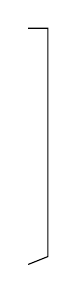
\begin{tikzpicture}
\draw (0,0)--(.25,0)--(.25,-2.9)--(0,-3);
\end{tikzpicture}}}
\diagram{\begin{tikzcd}[column sep=large]
\pi_1(X_{\bar y},\unsure{\xi}) \arrow[r,dash] &
\pi_1(X,\unsure{\xi}) \arrow[r] &
\pi_1(Y,\unsure{\eta}) \arrow[r] & 0
\end{tikzcd}}

\deleted{\unsure{Cela}}
généralise (\unsure{en dehors} l'hyp. noethérienne)
SGA IX 6.1, 6.2. \ldots\ Ne pas confondre avec les résultats de SGA X, où on prend une fibre \unsure{pas}%
\inserted{\uline{\unsure{néc|ici}}}%
\uline{générique} (en revanche, il y faut \unsure{je crois} que $f$ \unsure{soit} propre \ldots).
